\documentclass[11pt,a4paper,sans]{moderncv}

%% ModernCV themes
\moderncvstyle{casual}
\moderncvcolor{black}
\renewcommand{\familydefault}{\sfdefault}
\setlength{\hintscolumnwidth}{0.2\textwidth}
\nopagenumbers{}
\newcommand{\tab}{\hspace{0.3cm}}

\definecolor{blue}{rgb}{0.0,0.5,1.0}
\definecolor{orange}{rgb}{1.0,0.55,0.0}
\definecolor{green}{rgb}{0,0.8,0.25}
\definecolor{DarkOrchid}{rgb}{0.6, 0.2, 0.8}

%% Character encoding
\usepackage[utf8]{inputenc}

%% Adjust the page margins
\usepackage[inner=2.4cm,outer=2.4cm,top=2cm,bottom=3.5cm,scale=0.75]{geometry}
\usepackage{lscape}
\usepackage{pgfgantt}
\usepackage{xcolor}
%\usepackage{natbib}
\usepackage[english]{babel}
\usepackage[backend=biber,maxbibnames=99,dashed=false,style=authoryear,sorting=ydnt]{biblatex}%
\DeclareNameAlias{sortname}{last-first}
%\DeclareSortingScheme{noneyear}{
%	\sort{\citeorder}
%	\sort{\field{year}}
%}
\addbibresource{./CVbiblio.bib}
%\AfterPreamble{\hypersetup{colorlinks=false,linkbordercolor=red,pdfborderstyle={/S/U/W 1}}}

%% Personal data
\firstname{Cha\"im}
\familyname{De Mulder}
\title{}
\address{Gustaf Rydbergsgatan 5/1103}{217 55 Malm\"o -- Sverige}
\mobile{+32 479 74 55 02}
\email{demulderchaim@gmail.com}
%\homepage{www.johndoe.com}
\extrainfo{F\"odd 27/3/1991 i Gent}
\photo[76pt][0.8pt]{../images/ChaimDeMulderbis}
%\quote{Some quote (optional)}

%%------------------------------------------------------------------------------
%% Content
%%------------------------------------------------------------------------------
\begin{document}
\makecvtitle

%%%%%%%%%%%%%%%%%%%%%%%%%%%%%%%%%%%%%%%%%%%%%%%%%%%%%%%%%%%%%%%%%%%%%%%%%%%%%%
\vfill
\colorbox{orange!10}{
	\begin{minipage}{\textwidth}
		\section{\textcolor{orange}{\textbf{Arbetslivserfarenhet}}}
		\cventry{Oct. 2015 -- Mai 2019}{Doktorand}{\footnotesize Ghent University, Faculty of Bioscience engineering, Department of Data Analysis and Mathematical Modeling, BIOMATH group (Model based bioprocess analysis and optimisation)}{}{}{}
		\cvitem{}{\small $\bullet$ Utveckling av en software paket f\"or data behandling (\href{https://github.com/UGentBiomath/wwdata}{\underline{wwdata}})}
		\cvitem{}{\small $\bullet$ Modellbaserad st\"od av (investerings)beslut g\"allande avloppreningsverket i Eindhoven, Nederl\"anderna}
		%\cvitem{\centering\raisebox{-0.7\height}{
\includegraphics[width=0.12\textwidth]{../images/LogoUGent.png}}}{\small Modellbaserad st\"od av (investerings)beslut, \"okning av kunskap om och avancerad modellering av reningsverket i Eindhoven, Nederl\"anderna, i t\"at samarbete med operatorerna (Waterschap De Dommel).}
		\vspace{0.2cm}
		
		\cventry{Oct. 2014 -- Oct. 2015}{Forskningsassistent}{\footnotesize Ghent University, Faculty of Bioscience engineering, Department of Data Analysis and Mathematical Modeling, BIOMATH group}{}{}{}
		%\cvitem{\centering\raisebox{-0.7\height}{
\includegraphics[width=0.12\textwidth]{../images/LogoUGent.png}}}{\small Hydrodynamisk och biokinetisk modellering i sammanhang med High Rate Activated Sludge processen, i samarbete med Waterschap Brabantse Delta, Nederl\"anderna \newline}
		\vspace{0.2cm}
		
		%$\bullet$ Coupling a hydrodynamic model (using CFD) and a biokinetic model (using established wastewater treatment models) for the Wastewater Treatment Plant of Breda, The Netherlands.\newline
		%$\bullet$ Implementing a model for the simulation of the High Rate Activated Sludge Process, based on two previously described models.
		%\cventry{20/8/2014--12/11/2014}{PhD-scholarship application}{Ghent University, Faculty of Bioscience engineering, Department of Mathematical Modeling, Statistics and Bioinformatics, BIOMATH group (Model based bioprocess analysis and optimisation) and LabMET (Laboratory for Microbial and Environmental Technolgy)}{}{}{}
		%\cvitem{Project title}{Partial nitritation/anammox in mainstream: development based on hydrodynamic and kinetic modeling}
		%\cvitem{Project description}{\small Different control strategies to obtain Partial nitritation/anammox (PN/A) already exist in full-scale sidestream applications. In mainstream municipal wastewater treatment however, full-scale application has not been achieved, mainly due to hydrodynamic reactor-heterogeneity. The coupling of hydrodynamics (using CFD) and biokinetics (using established wastewater treatment models) offers a powerful way to gain insight in their interaction, and to move towards more solid design and control strategies, making full-scale PN/A implementation possible.}
		%\cvitem{\textcolor{green}{\underline{Skills}}}{Project preparation consisted of extensive literature research concerning CFD, wastewater treatment modeling, the PN/A process, the A/B-proces and multiple trial defenses}
		\cventry{2015--2019}{Engagemang som Young Water Professional (YWP) inom International Water Association (IWA)}{}{}{}{}
		%\cvitem{\centering\raisebox{-0.7\height}{
\includegraphics[width=0.07\textwidth]{../images/IWA}}\\}{\small 
			%Skaffade kunskaper 
			%$\bullet$ Activ inom styrelsen av den Belgiska avdelningen av IWA\newline
			%$\bullet$ Activ inom styrelsen av den IWA Specialist Group for Modeling and Integrated Assessment\newline
			%
			%$\circ$ Maintenance of \href{http://www.b-iwa.be}{\underline{website}}, \href{https://www.linkedin.com/groups?mostRecent=&gid=3760023&trk=my_groups-tile-flipgrp}{\underline{LinkedIn}}- and \href{https://twitter.com/BelgianIWA}{\underline{Twitter}}-account.\newline
			%$\circ$ Coordinator of the first, second and third \href{http://www.b-iwa.be/node/177}{\underline{B-IWA nocturnal}}
			%$\bullet$ co-organisator av IWA YWP Benelux Conference, Gent, Belgium, July 2017
		%}
		\vspace{0.2cm}
		\cventry{Jul. -- Aug. 2013}{Praktiktj\"anst i sammanhang med master thesis}{\footnotesize DC Water, Research and Development Department}{\footnotesize Washington DC, USA}{}{}
		%\cvitem{Title}{Researcher/MSc Student}
		%\cvitem{Description}{}
		%\cvitem{\textcolor{green}{\underline{Skills}}}{Operating successfully in a research working environment, team-work, critical analysis of research results}
		%\cvitem{\raisebox{-\height}{
\includegraphics[width=0.09\textwidth]{./LogoDCWater.png}}}
		%{\textbf{Project:} \small Batch experiments under different conditions to obtain AOB and NOB oxygen half-saturation constants through parameter estimation using a specific model describing the experimental procedure.}
		\vspace{0.2cm}
		
		\cventry{Jul. -- Aug. 2012}{IAESTE praktiktj\"anst}{\footnotesize Aalto University, Department of Biotechnology and Chemical Techno-logy}{\footnotesize Espoo, Finland}{}{}
		%\cvitem{Title}{Research assistant}
		%\cvitem{\raisebox{-\height}{
\includegraphics[width=0.08\textwidth]{./LogoAalto}}}
		%{\textbf{Project:} \small Catalysts used in the dehydration of xylose to furfural were characterized using micro-scale reactors, titration experiments and sugar-adsorption measurements.}
		%\cvitem{\textcolor{green}{\underline{Skills}}}{Working independently, soft/social skills: patience, open mind, communication}
		%\vfill
		%\vspace{0.5cm}
		
		
		%\cvitem{\raisebox{-\height}{
\includegraphics[width=0.08\textwidth]{./IWA.png}}}{\small
		%	$\bullet$ Co-organizer of an \href{http://www.iwarr2015.org/content/young-professionals-workshop-building-pipelines-resource-recovery}{\underline{IWA YWP Workshop}} (Aug 29 - 30, 2015)\newline
		%	$\bullet$ Assistant in the course Modeling and Control of Wastewater Treatment Plants, given at the Faculty of Bioscience Engineering, Ghent University.}
		
	%	\vspace{0.5cm}
	\end{minipage}
}
\vfill
%%%%%%%%%%%%%%%%%%%%%%%%%%%%%%%%%%%%%%%%%%%%%%%%%%%%%%%%%%%%%%%%%%%%%%%%%%%%%%
\colorbox{blue!10}{
	\begin{minipage}{\textwidth}
		\section{\textcolor{blue}{\textbf{Kunskaper}}}
		\cvitem{}{$\bullet$ \textbf{Engagerad milj\"o-ingenj\"or} med stort \textbf{analytiskt sinne} och breda intressen;\newline brinner mest f\"or \textbf{milj\"o- och klimatfr\aa gor.}}
		%\vspace{-.55cm}
		%\cvlistitem{Social och \textbf{storsint}}
		%\cvlistitem{Team-worker}
		\cvitem{}{$\bullet$ Stor fokus p\aa\ \textbf{effektivitet, struktur och entydig kommunikation} i b\aa de ensamt och samarbete}%, och d\"arf\"or ocks\aa\ van vid bra \textbf{time management}.}
		%\cvitem{}{$\bullet$ Grundl\"aggande kunskaper inom \textbf{project management}.}
		\cvitem{}{$\bullet$ Social och storsint.}
		\vspace{0.2cm}
		
		\cvitem{Software/IT}{$\bullet$ Avancerade: Python (allm\"an programspr\aa k), \LaTeX (ordbehandlingsprogram), WEST (modellering av avlopreningsverk)}
		%\vspace{-.55cm}
		\cvitem{}{$\bullet$ Grundl\"aggande: MS Office, Inkscape (ritprogram), Drupal (webbsidor)}
		%OpenFOAM, git(hub)
		\vspace{0.2cm}
		\cvitem{Spr\aa k}{
			\begin{tabular}{ll}
				$\bullet$ Nederl\"andska (modersm\aa l) & \tab $\bullet$ Engelska (flytande)\\
				$\bullet$ Svenska (avancerade) & \tab $\bullet$ Franska (grundl\"aggande)\\	
			\end{tabular}}
	\end{minipage}
}
\vfill
%%%%%%%%%%%%%%%%%%%%%%%%%%%%%%%%%%%%%%%%%%%%%%%%%%%%%%%%%%%%%%%%%%%%%%%%%%%%%%
\colorbox{DarkOrchid!10}{
	\begin{minipage}[]{\textwidth}
		\section{\textcolor{DarkOrchid}{\textbf{Utbildning}}}
		\cvitem{}{\textbf{Ghent University:}}
		\cventry{2012--2014}{Master i Bio-Science Engineering: Environmental Technology}{}{}{}{}
		\cventry{2009--2012}{Bachelor i Bio-Science Engineering: Environmental Technology}{}{}{}{} 
	\end{minipage}
}
\vfill


%%%%%%%%%%%%%%%%%%%%%%%%%%%%%%%%%%%%%%%%%%%%%%%%%%%%%%%%%%%%%%%%%%%%%%%%%%%%%%
\colorbox{green!10}{
	\begin{minipage}{\textwidth}
		\section{\textcolor{green}{\textbf{Ytterligare engagemang och meriterande aktiviteter}}}
		\cvitem{}{\footnotesize \textit{Klicka p\aa\ organisationens namn om du vill veta mer}}
		\cventry{2018--2019}{\href{http://climate-express.be}{\textbf{Climate Express..}}}{}{}{}{}
		\cvitem{\centering\raisebox{-0.6\height}{
\includegraphics[width=0.05\textwidth]{../images/ClimateExpress}}\\}{... som \"ar en grupp av volont\"arer som mobiliserar befolkningen f\"or en socialt r\"attvis \"overg\aa ng mot ett klimatneutralt samh\"alle.}
		\cventry{2018--2019}{\href{https://www.climateresponse.eu}{\textbf{Climate Response..}}}{}{}{}{}
		\cvitem{\centering\raisebox{-0.6\height}{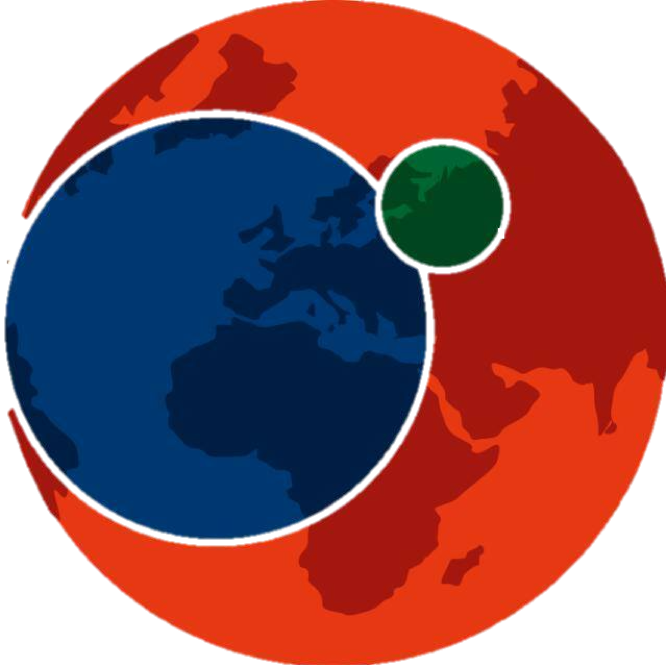
\includegraphics[width=0.05\textwidth]{../images/ClimateResponse}}\\}{... som l\"ar ut fakta om klimatf\"or\"andring och f\"ors\"oker p\aa verka debatten om klimatfr\aa gor fr\aa n en vetenskaplig infallsvinkel}
		\cventry{2018--2019}{\href{https://www.yaku.be}{\textbf{YAKU..}}}{}{}{}{}
		\cvitem{\centering\raisebox{-0.6\height}{
\includegraphics[width=0.06\textwidth]{../images/yaku.png}}\\}{... som siktar p\aa\ att simma i fl\"oderna i Gents innerstad. Citizen science \"ar v\aa r viktigaste hj\"alpmedel.}
		\cventry{2013--2018}{\href{https://iaeste.org}{\textbf{IAESTE..}}}{}{}{}{}
		\cvitem{\centering\raisebox{-0.6\height}{
\includegraphics[width=0.05\textwidth]{../images/iaeste_logo}}\\}{..., the International Association for the Exchange of Students for Technical Experience, som arrangerar praktiktj\"anster i \"over 80 l\"ander.}
		
		%\cvitem{2017--2018}{\textbf{Connect Region Project Coordinator}}
		%: \small Member of the Regional Management team of western Europe, day-to-day manamement of regional affairs. Responsible for several projects with participants from across the region.
		%\cvitem{}{ \normalsize}
		%\cvitem{2016--2017}{\textbf{LC Ghent Exchange Coordinator}}
		%: \small Board member of the Local Committee of Ghent, day-to-day management of a 25-person team of students. Resposible for international internship exchange and networking, jobraising.
	    %\cvitem{}{ \normalsize}
		%\cvitem{2015--2016}{\textbf{LC Ghent Vice-President \& Summer Reception Officer}}
		%\cvitem{}{\normalsize}
		%: \small General support on local level (team management)  and within international IAESTE groups (Region of western Europe). Jobraising and organizing activities for incoming trainees.
		%\cvitem{2014--2015}{\textbf{LC Ghent supporting member \& Summer Reception Officer}}
		%: \small Design of PR materials, presenting IAESTE to companies, jobraising. Organizing activities for incoming trainees. 
		%\cvitem{}{\normalsize}
		%\cvitem{2013--2014}{\textbf{LC Ghent Secretary}}
		%: \small Responsible for meeting reports, jobraising. 
		%\cvitem{}{\normalsize}
		%\vspace{0.5cm}
		\cvitem{}{\textbf{Kurser}}
		\cvitem{14/9/2015 -- 13/11/2015}{MOOC by the Stockholm Resilience Center: \textit{Planetary Boundaries and Human Opportunities: the quest for safe and just development on a resilient planet}}
		\vspace{0.2cm}
		\cvitem{9/7/2019 -- 11/7/2019}{Coppieters Academy course: \textit{Climate Action in a Changing Europe}}
		\vspace{0.2cm}
		\cvitem{}{\textbf{Idrott och andra intressen}}
		\cvitem{}{Friidrott, s\"allskapsspel, Nordisk kultur.}
		%\cvitem{}{\textbf{General interests}}
		%\cvitem{}{Music, climate related, environmental and social issues, Scandinavian culture}
		%\cvitem{}{Open Source initiatives}
		%\cvitem{}{Climate related and environmental issues}
	\end{minipage}
}
\vfill

%%%%%%%%%%%%%%%%%%%%%%%%%%%%%%%%%%%%%%%%%%%%%%%%%%%%%%%%%%%%%%%%%%%%%%%%%%%%%%
\begin{center}
	\begin{ganttchart}[
		%hgrid=true,
		%vgrid=true,
		y unit title=0.8cm,
		y unit chart=0.5cm,
		x unit=0.6cm,
		bar1/.style={bar/.append style={fill=blue}},
		bar2/.style={bar/.append style={fill=orange}},
		bar3/.style={bar/.append style={fill=green}},
		bar4/.style={bar/.append style={fill=DarkOrchid}}
		]{1}{16}
		\scriptsize
		\ganttset{group height=0.5cm}
		\gantttitle{2012}{2} \gantttitle{2013}{2} \gantttitle{2014}{2} \gantttitle{2015}{2} \gantttitle{2016}{2}\gantttitle{2017}{2}\gantttitle{2018}{2}\gantttitle{2019}{2}\\
		\textcolor{DarkOrchid}{\ganttbar[bar4]{Master}{1}{5}}\\
		\textcolor{orange}{\ganttbar[bar2]{IAESTE Praktiktj\"anst}{2}{2}}\\
		\textcolor{orange}{\ganttbar[bar2]{DC Water Praktiktj\"anst}{4}{4}}\\
		\textcolor{orange}{\ganttbar[bar2]{Forskningsassistent}{6}{7}}\\
		\textcolor{orange}{\ganttbar[bar2]{Doktorand}{8}{15}}\\
		\textcolor{orange}{\ganttbar[bar2]{IWA engagemang}{7}{15}}\\
		\textcolor{green}{\ganttbar[bar3]{IAESTE medlem}{3}{13}}\\
		\textcolor{green}{\ganttbar[bar3]{Climate Response}{14}{15}}\\
		\textcolor{green}{\ganttbar[bar3]{Climate Express}{14}{15}}\\
		\textcolor{green}{\ganttbar[bar3]{YAKU}{14}{15}}\\
		%\textcolor{green}{\ganttbar[bar3]{IAESTE support}{14}{16}}\\
		%\textcolor{green}{\ganttbar[bar3]{IAESTE Vice President}{14}{16}}\\		
		\textcolor{green}{\ganttbar[bar3]{Friidrott}{1}{15}}\\
		\textcolor{blue}{\ganttbar[bar1]{Kv\"allskurser Svenska}{6}{15}}
		%\textcolor{green}{\ganttbar[bar3]{IAESTE support}{14}{16}}\\
		%\textcolor{green}{\ganttbar[bar3]{IAESTE Vice President}{14}{16}}\\		
		\normalsize
	\end{ganttchart}
\end{center}
\vfill


%\newpage

%%%%%%%%%%%%%%%%%%%%%%%%%%%%%%%%%%%%%%%%%%%%%%%%%%%%%%%%%%%%%%%%%%%%%%%%%%%%%%
%\section{Personal}
%\cvitem{}{I am a \textbf{motivated and enthusiastic} young man, looking for a \textbf{challenging and diversified} job. During both my working experiences so far, I found that contact with colleagues is something I really appreciate. I am convinced that \textbf{working in a team} with people of different backgrounds can yield better results and more creative engineering solutions.\newline Since I believe I have \textbf{strong values}, I am looking for an employer whose vision I can easily identify with. It goes without saying that I will be even more eager to show a \textbf{committed engagement} working for a company that appeals to me.}

%Obviously, I am ready to show a \textbf{commited engagement} in such a context. }
%\cvitem{Looking for}{Challenging and diversified job, team-work, employer vision and mission I can identify with}
%%%%%%%%%%%%%%%%%%%%%%%%%%%%%%%%%%%%%%%%%%%%%%%%%%%%%%%%%%%%%%%%%%%%%%%%%%%%%%
%\section{Attended meetings and conferences}
%\cvitem{}{\textbf{EU COST-Action meeting}, \textit{Paris}, /3-/4/2015: represent the research group professor in working group on modeling for decision support.}
%\cvitem{}{\textbf{Resource Recovery Conference 2015},\textit{Gent}, /9/2015-/9/2015}
%\cvitem{}{\textbf{IAESTE Annual Conference},\textit{Prague}, 22/1/2016-29/1/2016}


%%%%%%%%%%%%%%%%%%%%%%%%%%%%%%%%%%%%%%%%%%%%%%%%%%%%%%%%%%%%%%%%%%%%%%%%%%%%%%
%\section{\textbf{Scientific publications}}
%\renewcommand{\section}[2]{}

%\subsection{Journal papers}
%\nocite{*}
%\printbibliography[type=article,title={Journal papers}]
%\printbibliography[type=inproceedings,title={Conference papers (presentations and posters)}]%,sorting=noneyear]
%\printbibliography[type=manual,title={Software}]%,sorting=noneyear]
%
%\newpage
%\section{\textbf{Scientific conferences}}
%\cvitem{{\centering Apr. 2--6, 2016}}{IWA/WEF Wastewater Treatment Plant Modeling seminar (WWTMod)\newline Annecy, France, Workshop co-organizer}
%
%\cvitem{May 21--24, 2017}{Frontiers International Conference on Wastewater Treatment (FICWTM) \newline Palermo, Italy, Oral presentation}
%
%\cvitem{June 11--14, 2017}{IWA Specialized Conference on Instrumentation, Control and Automation (ICA) \newline Qu\'ebec City, Canada, Oral presentation (not present at the conference)}
%
%\cvitem{July 5--7, 2017}{Young Water Professionals BeNeLux conference \newline Ghent, Belgium, Oral presentation}
%
%\cvitem{Nov. 7--9, 2017}{IWA Conference on sustainable Wastewater Treatment and Resource Recovery: Research, Planning, Design and Operation (NRR-LWWTP)\newline Chongqing, China, Oral presentation}
%
%\cvitem{Mar. 10--14, 2018}{IWA/WEF Water Resource Recovery Modelling Seminar (WRRMod)\newline Qu\'ebec City, Canada, Poster presentation}
%
%\cvitem{Sept. 16--21, 2018}{IWA World Water Congress and Exhibition\newline Tokyo, Japan, Poster presentation (not present at the conference)}
%
%\section{\textbf{Educational activities}}
%\cvitem{Teaching}{
%	$\bullet$ Assisting with the Master course Modeling and Control of Wastewater Treatment Plants
%}{}{}{}{}
%\cvitem{MSc student guidance}{
%	$\bullet$ Katrien Couchez: Modeling the effect of urine separation on full-scale Waste Water Treatment Plant operation.\newline
%	$\bullet$ Vincent Van De Maele: The impact of fluctuating energy prices on WWTP cost optimisation\newline
%	$\bullet$ Tom Lauriks: Opportunities and limitations of connecting Life Cycle Assessment to a dynamic wastewater treatment plant model
%}{}{}{}{}


\end{document}